\chapter{Aquifer test}
\label{chapter:Fieldwork_data_analysis}

The performance of an ASR system is dependent on the physical properties of its surroundings \citep{Bakker2010}. In the north of Ghana, subsurface characteristics can vary at short mutual distances  \citep{Owusu2017}. Representative information on the local geohydrology is obtained through site-specific measurements. Aquifer tests are performed at multiple locations in northern Ghana. \\
The research locations are presented in Section \ref{section:research_locations}. Section \ref{section:Methods_fieldwork} describes the aquifer test methodologies in measurement set-up and data analysis. Appendix \ref{chapter:fieldworkresults} contains the raw measurement results. The aquifer test data is analysed in Section \ref{section:TS}. In Section \ref{section:fieldwork_conclusions} the conclusions on the site visits and the data analysis are described. The chapter concludes with the derivation of locally applicable values for $T$ and $S$. These parameters are the input for the study on potential ASR system improvements in northern Ghana. 
%
% In this research perspective, multiple northern Ghana borehole locations are subjected to groundwater pumping tests. 
%This sections explains.. and derives More details on the results of all 
%
%A selection of fit solutions is presented by location in section \ref{section:TS}. 
%Detailed information on the equipment that was used, the set-up of the pumping tests as well as the monitoring of an operating ASR system can be found in Appendix \ref{chapter:fieldwork_set-up}. The obtained raw fieldwork data can be found in the site-specific fact-sheets of Appendix \ref{chapter:fieldworkresults}. The purpose of this fieldwork is to determine geohydrological subsurface parameters, transmissivity ($T$) and storativity ($S$), which are used as input for further investigation into upscaling these systems. 
%
%%This chapter contains the analysis of gathered fieldwork data. First, the methodology for data analysis, including some theoretical background, is explained (Section \ref{section:derivation_methods}). Section \ref{section:TS} contains the derivation of the local geohydrological parameter values: $T$ and $S$. Finally, the chapter concludes with the determination of parameter bandwidths (Section \ref{section:fieldwork_results}), which will be used in the subsequent model simulations. 
%
%It might seem trivial, but the functioning of an ASR system is dependent on its surroundings. The locally applicable soil parameters ($T$ and $S$) have to be determined for the research follow-ups. The desired information is obtained by the application of site-specific measurements within northern Ghana. The Fieldwork set-up strategies as well as the approaches in data analysis are included in the methodology (Section \ref{section:Methods_fieldwork}). The answers to the sub-question are generated in Chapter \ref{chapter:Fieldwork_data_analysis}.} 
%
%This section contains the conclusions that can be drawn from the site visits and the analysis of pumping test data. The final part of this section describes how this data was used to derive parameters for scenarios to study potential methods for improvements of ASR systems in northern Ghana.  \\

\section{Research locations in northern Ghana}
\label{section:research_locations}
Multiple ASR systems are present in the Upper East Region (UER) and the Northern Region (NR) of Ghana. Commissioned by the NGO Conservation Alliance (CA), some of these systems are installed in the summer of 2016. Pumping tests are performed at four (CA) ASR systems, located in Bingo; Nungo; Nyong Nayili and Janga. At the location Ziong an ASR system is used for the monitoring of the system practical use by farmers. Figure~\ref{fig:Overviewlocations} shows a map of the research locations in northern Ghana. \\

\begin{figure}[ht]
 \centering
 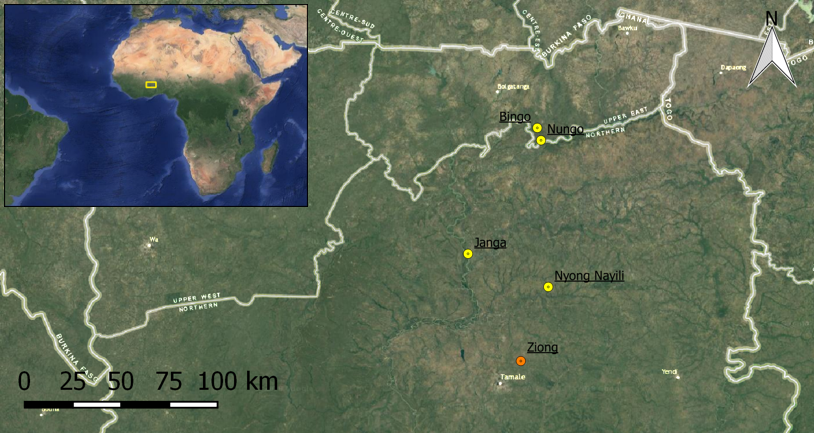
\includegraphics[width=\linewidth]{Overview_locations_northern_Ghana}
 \captionsetup{justification=centering} 
 \caption{The northern Ghana research locations}
 \label{fig:Overviewlocations}
\end{figure}

%\section{Methods - Test set-up \& analysis}
\section{Methods - Set-up \& analysis}
\label{section:Methods_fieldwork}
The five northern Ghana study sites (Section \ref{section:research_locations}) are subjected to aquifer tests. A complete description of the test process (from measurement data generation to geohydrological parameter values derivation) is described below. The raw results (measurement data) can be found in Appendix \ref{chapter:fieldworkresults}. Data analysis (Section \ref{section:TS} \& \ref{section:fieldwork_conclusions}) is possible by the implementation of the here presented methodologies.

\subsection{Measurement set-up}
\label{subsection:measurement_structure}
This section contains the ins and outs of the practical aquifer test set-up. The aquifer tests accommodates both pumping-recovery tests and the monitoring of the system use by farmers. Due to differences in ASR systems encountered, the data collection is designed by a hybrid measurement approach. The stated approach can be used as input for data (re)production (transparency). \\

\textbf{Pump installation} \\
Based on the (2016) original log sheets (Appendix \ref{chapter:Borehole_logsheets}), site-specific borehole depths are known in advance. The ASR system inspection showed, the accumulation of sedimentation at the borehole bottom. To prevent pump damages and make sure properly functioning is maintained, actual borehole depths are measured before pumping tests are executed. Outcomes of the measurements are taken into account for each individual set-up. To prevent the excessive spread of soil particles, the submersible pump is positioned at least 5 m above the measured borehole bottom (sediment). In practice, this resulted in a pump suction depth of approximately 30-35 m.
\bigskip \\
\textbf{Pump discharge \& measurement} \\
A single 100 m hose is directly connected to the outlet of the submersible pump. Based on the pump position (deep inside borehole), a distance of circa 65 m is applied for the horizontal displacement of water. At this distance, water is discharged on the surface. The head of the hose is equipped with a nozzle to roughly regulate the discharge rate. By the use of this nozzle, discharge rates in the range of 50-75 m$^{3}$/d are obtained during the pumping tests. Rates are measured by the use of a stopwatch and a 50 l bucket. Starting at the moment of pump operation, the duration of filling is measured twice every 15 minutes. The obtained 15 minute average is used to calculate the time dependent discharge rates. More detailed discharge information can be found in the site-specific fact sheets (Appendix \ref{chapter:fieldworkresults}).
\bigskip \\
\textbf{Groundwater table (GWT) measurement} \\
Groundwater level reductions caused by pumping tests are preferably measured in multiple piëzometers, located at a certain known horizontal distance from the discharge well \citep{Kruseman2000}. In the northern Ghana surroundings, close range monitoring options are absent. Due to a lack of time and/or resources these facilities could not be arranged either. Moreover, the implementation of such facilities do not match research nature. Aim of this research is to collect fieldwork data by the use of minimal resources. The absence of widespread measurement options strengthens this approach. As a consequence, the time dependent GWTs (drawdowns) are measured in the discharge well only. \\
A water tape is used as hand equipment. First of all to determine the initial (static) GWT. Subsequently, the device is applied as a real time indicator of drawdown. During the pumping tests, multiple hand measurements are applied at randomly picked moments to monitor the test progress. Gathered data functions as verification and back-up of the pressure sensors (divers), which are normative. \\
Two types of divers (different brands) are used as GWT measurement devices. Product specifications show that these divers can respectively measure pressures up to 10 m (Van Essen) and 9 m (In-Situ) water column (Appendix \ref{chapter:fieldwork_set-up}). The northern Ghana regional subsurface is characterized as highly heterogeneous. The pumping test GWT drawdown magnitude is therefore unpredictable. To prevent the occurrence of missing drawdown data, the single borehole is equipped with multiple divers at ascending depths. The water column between the initial static water table and pump position is filled with about four divers, with a mutual distance that meets the divers range specifications. To make sure the divers stay in position they are leashed to a rope which runs from well top to pump. This measurement set-up forms a robust network for the collection of drawdown data (figure~\ref{fig:general}). \\
However, practical circumstance can cause the application of a more simplistic set-up (figure~\ref{fig:simplified}). One can think of a situation in which the pump is already installed and/or will not be removed at the end of the pumping test. In this case, the (rope) attachment of the divers to the pump is not possible. Adverse effect of the simplistic set-up is a more vulnerable data collection. To prevent the occurrence of undesired diver movement, a minimum distance of 5-10 m between the pump and lowest diver is implemented in this set-up. A complete overview of the borehole measurement set-up (general and simplistic) can be found in figure~\ref{fig:set-up}. \\

\begin{figure}[h]
	\centering
	\begin{subfigure}[b]{0.4\linewidth}
		\centering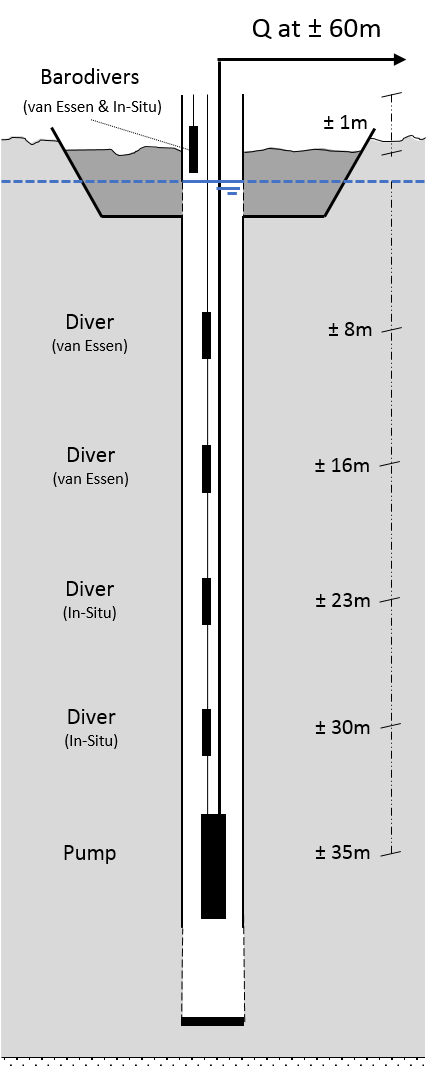
\includegraphics[width=0.65\linewidth]						{Setup_pumping_test.png}
		\captionsetup{justification=centering}		
		\caption{\label{fig:general}}
		\end{subfigure}%\hfill
	\begin{subfigure}[b]{0.4\linewidth}
        \centering\includegraphics[width=0.65\linewidth]						{Setup_pumping_test_bingo.png}
		\captionsetup{justification=centering}		
		\caption{\label{fig:simplified}}
		\end{subfigure}
	\captionsetup{justification=centering}	
	\caption{Fieldwork (measurement) set-up (\subref{fig:general}) general, ~(\subref{fig:simplified}) simplistic} 
	\label{fig:set-up}
\end{figure} 

Besides the divers, the measurement set-up also accommodates two baro-divers (van Essen \& In-Situ). The baro-divers are positioned in the borehole top section. Drawdown is by definition expressed as time dependent GWT reductions relative to the initial status. Short-term atmospheric fluctuations in pressure are compared to the water pressures negligible small. Nonetheless, these minor atmospheric influences are also included in the data collection. 
\bigskip \\
\textbf{Pumping test duration \& time measurement} \\
For each individual pumping test the exact start of pump operation could not be determined in advance. As a consequence, the total pumping test duration differs per pumping test as well. In every single measurement, a minimum of four hours of pumping and one hour of recovery is pursued. \\
To avoid unnecessary risks in missing out on the collection of drawdown data, all pressure sensors are programmed to start logging in time (08:00:00, local time, at pumping test days). All divers are set to log with a similar linear interval of 10 seconds. As a single exception, the In-Situ BaroTROLL is programmed to linear log once a minute (its minimum sample interval). \\

* An overview of the aquifer test results for each individual research location can be found in Appendix \ref{chapter:fieldworkresults}. More details on the applied equipment can be found in Appendix \ref{chapter:fieldwork_set-up}.

\subsection{Data analysis}
\label{subsection:derivation_methods}
Raw drawdown time series are the result of in-field measurements. The data sets are more or less meaningless on its own. The methods below describe the required components in analysis to transforms the obtained aquifer test data to the desired transmissivity ($T$)and storativity ($S$) values. \\

\textbf{Simplified theoretical models} \\
The original borehole log sheets (appendix \ref{chapter:Borehole_logsheets}) are the most reliable source of local geological information available. Although the sheets contain site-specific information, similarities in stratification are present. In each case (\ref{section:research_locations}) the upper 50 m is divided into two or three layers, consisting of a (semi-)impermeable top layer and below that one or two high(er) permeable layers (aquifers). Groundwater tables are predominantly positioned slightly below the bottom of (semi-)impermeable layer, in the top aquifer (labelled as layer 1 in the figure below). Strictly seen, the conditions are therefore unconfined. But given the small interval (relative to total model thickness) between the the aquifer top and the GWT, the situation is close to confined. Based on the borehole log sheets three simplified theoretical models for the analysis of fieldwork data are proposed, as depicted in Figure \ref{fig:schematic_fieldwork_analysis}. 

\begin{figure}[h!]
	\centering
	\begin{subfigure}[b]{0.21\linewidth}
		\centering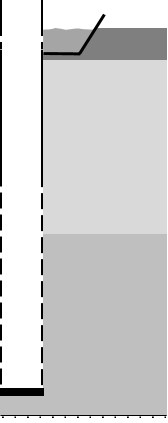
\includegraphics[width=0.6\linewidth]{Schematic_general_analysis}
		\captionsetup{justification=centering}		
		\caption{\label{fig:Schematic_general_analysis}}
		\end{subfigure}%\hfill
	\begin{subfigure}[b]{0.12\linewidth}
		\centering
\includegraphics[width=0.6\linewidth]{arrow_right}
		\end{subfigure}%\hfill
		%{\LARGE$\yrightarrow{}$}
	\begin{subfigure}[b]{0.21\linewidth}
		\centering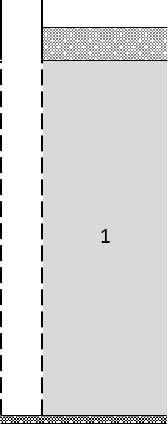
\includegraphics[width=0.6\linewidth]{Schematic_1lay_analysis}
		\captionsetup{justification=centering}		
		\caption{\label{fig:Schematic_1lay_analysis}}
		\end{subfigure}%\hfill
	\begin{subfigure}[b]{0.21\linewidth}
        \centering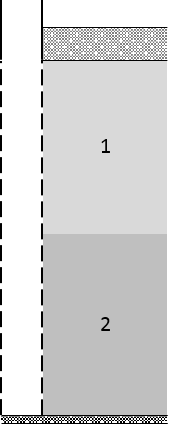
\includegraphics[width=0.6\linewidth]{Schematic_2lay_analysis}
		\captionsetup{justification=centering}		
		\caption{\label{fig:Schematic_2lay_analysis}}
		\end{subfigure}
	\begin{subfigure}[b]{0.21\linewidth}
        \centering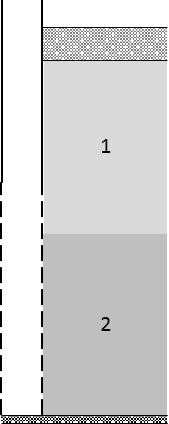
\includegraphics[width=0.6\linewidth]{Schematic_3lay_analysis}
		\captionsetup{justification=centering}		
		\caption{\label{fig:Schematic_3lay_analysis}}
		\end{subfigure}
	\captionsetup{justification=centering}	
	\caption{Schematic cross-sectional view of (\subref{fig:Schematic_general_analysis}) generalized northern Ghana soil stratification and simplified representations: (\subref{fig:Schematic_1lay_analysis}) a single layer system, ~(\subref{fig:Schematic_2lay_analysis}) a double layer system, and ~(\subref{fig:Schematic_3lay_analysis}) a system with two layers and partial penetration of the well} 
	\label{fig:schematic_fieldwork_analysis}
\end{figure} 

These simplified models (Figure \ref{fig:Schematic_1lay_analysis} - \ref{fig:Schematic_3lay_analysis}) mimic local conditions, making the derivation of representative hydraulic subsurface characteristics ($T$ and $S$) potentially possible \citep{Kruseman2000}. Double layered models are applied to provide more degrees of freedom, perhaps resulting in more accurate solutions. To limit the chances of equifinality (abundant degrees of freedom) a maximum of two soil layers are implemented in data analysis. \\ 

\textbf{Parameter derivation method's \& model environment} \\
It lacks a single best approach in the derivation of the geohydrological parameter values ($T$ and $S$). A widespread variety of analyses (e.g. analytical and computational) can be applied on the pumping test data. The details of the (analytical) models and methods used in this research are described below.

\begin{itemize}
\item{Theis's method} \\
Groundwater drawdown due to the withdrawal of water can be determined analytically with Theis's equation (Equation \ref{eq:theis}). Theis's method is applicable on the situation depicted in Figure  \ref{fig:Schematic_1lay_analysis}; a constant rate pumping test applied on a well that is fully penetrating a single layer aquifer \citep{Kruseman2000}. Confined conditions are assumed in Theis's method. Therefore, this analytical solution is suitable for obtaining a first indication (approximation) of the research geohydrological parameters.   
\end{itemize}


\begin{equation}
\label{eq:theis}
 s = \frac{Q}{4\pi K D} E_1(u)
\end{equation}

\begin{equation}
 u = \frac{r^{2} S}{4 K D t}
\end{equation}

Where $s$ (m) is the drawdown at distance $r$ (m) from the well, $Q$ (m$^{3}$) is the constant well discharge , $KD$ (m$^{2}$/d) is the aquifer transmissivity ($KD$ = $T$), $S$ (-) is the aquifer storativity, $t$ (d) is the time measured from the start of pumping and $E_1$ is the exponential integral. The drawdown measurements in this research are limited to in-well measurements. The distance $r$ in Theis's equation is assumed to be the length of the well radius (0.0635 m). Appendix \ref{sec:python_analysis} shows the implementation of Theis's method in Python.

\begin{itemize}
\item{Analytic Element Modelling in TTim} \\
TTim is a computer program based on analytic elements and designed for the analysis of transient groundwater flow. The analysis can be applied on a single or multiple layer(s). Several analytical elements (and types of elements) can be added to model layers. The use of TTim makes it possible to take additional well characteristics into account. Groundwater heads can be determined inside the well and the model optionally accounts for borehole storage and well skin resistance. Moreover, well discharge can be toggled on and off multiple times. This allows for simulations of both single pumping-recovery tests and long-term well operations \citep{Mishra2013,Bakker2013}. \\

This research fieldwork data is analysed within the TTim \texttt{Model3D} configuration. A single well (analytical element) is included in the model environment. The groundwater heads are determined inside the well. Aspects as actual borehole storage, optimal borehole storage and/or optimal well resistance are alternately accounted in different compositions of analysis. Moreover, the three types of simplified theoretical models (Figure \ref{fig:schematic_fieldwork_analysis}) are consecutively considered. A complete overview of all approaches in data analysis (25x) can be found in Appendix \ref{sec:data_analysis overview}. \\

The top layer (aquifer 1 in Figure \ref{fig:schematic_fieldwork_analysis}) is configured as being a phreatic layer. In other words, the top layer storage coefficient ($S$) is a phreatic storage coefficient ($S_y$). This model assumption is based on the observed initial groundwater tables, which are located below the bottom of the (semi-)impermeable top layer. In analysis, each simplified model layer has a hypothetical thickness of 1 m. The derived hydraulic conductivities ($k$) can therefore be interpreted as transmissivities ($T$) and the storage is expressed as the layer storage coefficient ($S$). This is done to directly derive $T$ and $S$ values. Additionally, this approach automatically corrects for the absence of knowledge on the thickness of the deepest soil layer in which the well is screened. There is no information about soil conditions beyond the bottom of the wells in the borehole log-sheets (Appendix \ref{chapter:Borehole_logsheets}). \\
\end{itemize} 

\textbf{Optimization functions} \\
As a final step in the determination of values for $T$ and $S$, the analytical solution (Theis's method) and composed TTim models are linked (fitted) to the fieldwork data. Two optimization functions are applied.

\begin{itemize}
\item{Fmin-RMSE function} \\
Differences between the measured and modelled drawdown (curves) can be expressed by the Root-Mean-Square-Error (RMSE) objective function (Equation \ref{eq:RMSE}). The \texttt{Fmin} function (part of Python's \texttt{scipy.optimize} package) is applied to minimize the RMSE value. In other words, the function is applied to minimize the difference between modelled and observed drawdowns. The optimization results in (RMSE based) optimal $T$ and $S$ values (and optionally values for borehole storage and/or well skin resistance). These values theoretically represent local conditions. An example Python implementation of the \texttt{Fmin-RMSE} optimization function is depicted in Appendix \ref{sec:python_analysis}. 
\end{itemize}
% example of monospace use: \texttt{hier wat je wilt hebben in monospace}!

\begin{equation}
\label{eq:RMSE}
 RMSE = \sqrt{\Sigma\frac{(s_{mod}-s_{field})^{2}}{N}}
\end{equation}

Where $s_{\text{mod}}$ is the modelled drawdown (m), $s_{\text{field}}$ is the observed drawdown (m) and N is the number of data points. \\
 
\begin{itemize}
\item{Calibration function} \\
TTim has a built-in calibration function for the derivation of parameter values. Application of this second method improves the research robustness (reference values). An example of the Python implemented TTim \texttt{Calibrate} optimization function is part of Appendix \ref{sec:python_analysis}. \\
\end{itemize}

Both optimization methods require initial parameter estimations. More than one suitable solution is possible, which makes the outcome of the optimization dependent on the choice of the initial values. Other studies found that $T$ and $S$ values are commonly low in northern Ghana \citep[e.g.][]{Owusu2015,Owusu2017}. Based on these other studies the following initial conditions are applied: $k_{aq0}$ is 10 (m/d), $k_{aq1}$ is 10 (m/d), $S_{aq0}$ is 0.01 (-), $S_{aq1}$ is 0.001 (-) and well resistance is 0.1 (d). The well radius (measured in-field) is used as the (initial) borehole storage: 0.0635 (m). Boundary conditions are applied to avoid the optimization resulting in physically improbable parameter values, i.e. negative parameter values and unnaturally high storativity values (greater than 0.3 (-)). \\

%(write something over initial conditions. Such small values. Not one single best solution. multiple 'best' solutions potentially close to each other. so solutions highly influential by the arbitrary chosen initial conditions. For each location several attempts done to see which initial conditions score pretty good. And subsequently generalization of those initial parameters applied per location/pumping test. for example better fit at Bingo at initial condition for T (KD) of 10, 10 (lay one and two) for fmin then for cal (2 layered system.) But 2 layered system all of sudden scores better with initial conditions 5, 1 for example.  

%This section contains the conclusions that can be drawn from the site visits and the analysis of pumping test data. The final part of this section describes how this data was used to derive parameters for scenarios to study potential methods for improvements of ASR systems in northern Ghana.

\section{Data processing}
\label{section:TS}
The findings of the site visits are described in this section. Moreover, the section contains the analysis of the aquifer test data. The most important outcomes for each of the five locations are discussed below. A complete overview of all simulations in data analysis (25 per location) can be found in Appendix \ref{chapter:Extense_fieldwork_analysis}.  
% methods in fieldwork data analysis and models mentioned in the previous section are applied on the measurements from the five locations: Bingo, Nungo, Nyong Nayili, Janga and Ziong. The measurement results are included in the fact-sheets of Appendix \ref{chapter:fieldworkresults}. 

\subsection{Location: Bingo}

\textbf{Site inspection}\\
The surroundings of Bingo are characterized by a mildly sloping landscape. (Bed)rock appears occasionally at the surface. Site inspection showed an abundance of charred vegetation. The area is exposed to bush fires. As a consequence of these bush fires the agricultural field is not in operation. Map inspection shows the presence of the Volta river within several kilometres from Bingo. However, no indications of surface water (water-bodies and/or ponds) were observed. Bingo inhabitants experience inundation levels up to 1-2 m, usually lasting for days. The inhabitants label wet season flooding as high. Flooding is not always directly caused by rain. Sometimes rainfall collects to fill up depressions in the landscape at a certain moment in time. Inspection on the infiltration well revealed the presence of a steel lid. Above surface level no well screen perforations were observed. \\

\textbf{Measurement quality}\\
A malfunctioning power converter postponed the pumping test start. Since nightfall was a time limiting factor, the delay resulted in a shortened total test duration. Well turbulence caused the rope to which the divers were tied to tangle, which meant the sensor depths changed over the course of the experiment (see measurement set-up in Appendix \ref{chapter:fieldwork_set-up}). Additionally, because of the tangle, hand measurements also became unreliable. The direct result is a long-term gap in pumping test drawdown data (yellow dotted line in Figure \ref{fig:Bingo_best}). The exact drawdown at the last moment of pumping is missing. \\

\textbf{Fit analysis} \\
The absence of data has its effects on the parameter fitting capabilities. As visible in Figure \ref{fig:Bingo_best}, Theis's method encounters difficulties here. Drawdown most definitely exceeded the measurement limit of 8 m. This is not reflected in the parameter outcome of Theis's method. Defective fitting capabilities, due to a gab in data, are clearly less emphatically present in the analysis by the use of TTim.  Optimal parameter values are found at which drawdown curves exceed the drawdown measurement limit. Taking borehole storage and/or well resistance in consideration may potentially underlie this. This example shows it is not by definition required to feature complete drawdown data. By the use of TTim incomplete time series can result in adequate optimal parameter values. In order size the values found are low but align initial conditions. Furthermore, it can be appointed that the double-layered transmissivity values found, suggest the presence of only one layer of groundwater flow. \\

\begin{table}[h!]
\small
\centering
\caption{Bingo - overview best fit parameters}
\label{tab:bing_table}
\begin{tabular}{l|c|r|r|rr|rr|c}
\hline 
\textbf{}       & \textbf{Method} & \textbf{Stor [m]} & \textbf{Res [d]} & \textbf{T1}  & \textbf{T2   [m$^2$/d]}  & \textbf{S1}  & \textbf{S2 [-]}  & \textbf{RMSE [m]} \\ \hline \hline
Analytical                & fmin             & -             & -            & 10.83      & -          & 2.0e-04    & -          & 0.798 \\
1 lay                     & fmin             & 0.0647        & 5.6e-02      & 26.23      & -          & 6.6e-03    & -          & 0.163 \\
2 lay                     & fmin             & 0.0635        & -            & 2.8e-04    & 8.25      & 3.0e-03    & 2.1e-06    & 0.107 \\
2 lay (pp)                & fmin             & 0.0597        & -            & 8.6e-04    & 7.44      & 7.1e-03    & 6.3e-06    & 0.078 \\ \hline    
\end{tabular}
\end{table}

\begin{figure}[h!]
 \centering
 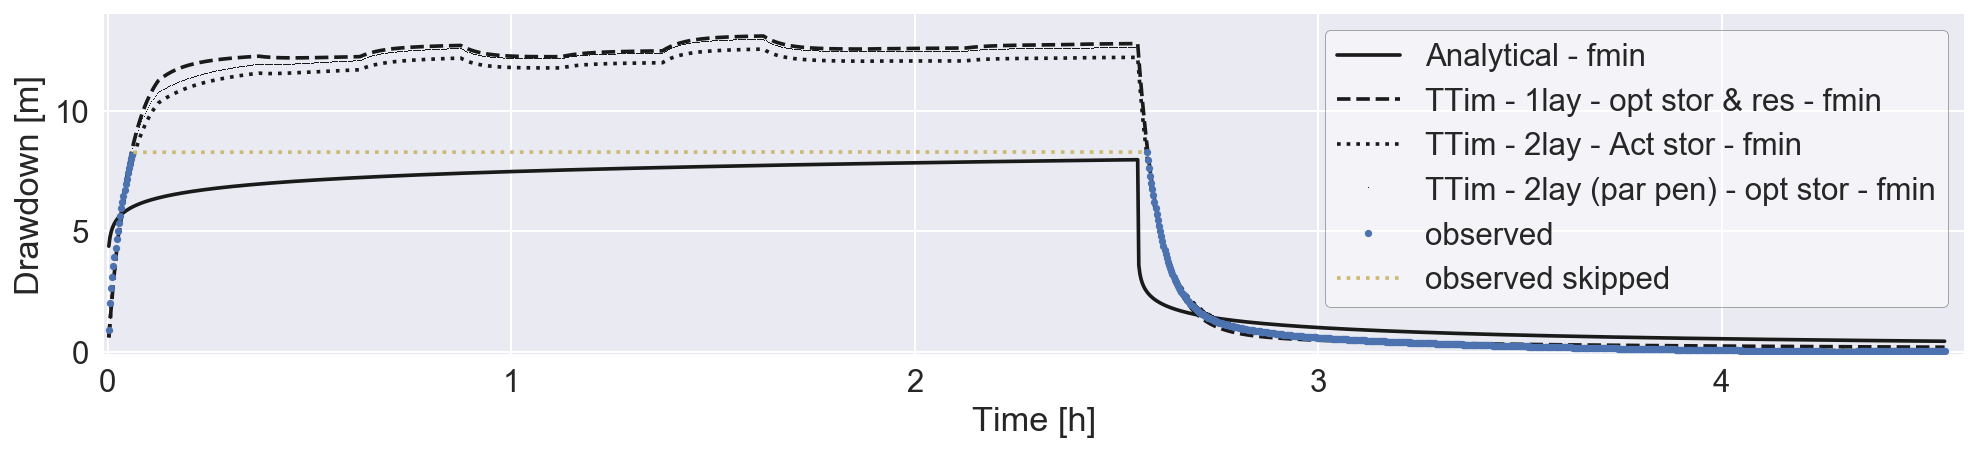
\includegraphics[width=\linewidth]{bingo_multi_lay_best}
 \captionsetup{justification=centering} 
 \caption{Bingo - Simplified models best fit}
 \label{fig:Bingo_best}
\end{figure}

\textbf{Effect of model complexity} \\
Both parameter optimization functions (\texttt{Fmin} and \texttt{Calibrate}) are able to derive reasonable solutions. Results of the \texttt{Calibrate} optimization function reveal that an increase in model degrees of freedom does not necessary leads to better performance (Appendix \ref{chapter:Extense_fieldwork_analysis}). By looking at the TTim best fit solutions (Figure \ref{fig:Bingo_best}) only minor distinction can be made in the performance between the models with a single layer, double layer or double layer with a partially penetrating well. Overall, model accuracy slightly increases (Root-Mean-Square-Error slightly decreases) with an increase in model complexity. However, this increase is not significant.

%\begin{figure}[h!]
%	\centering
%	\begin{subfigure}[b]{1\linewidth}
%		\centering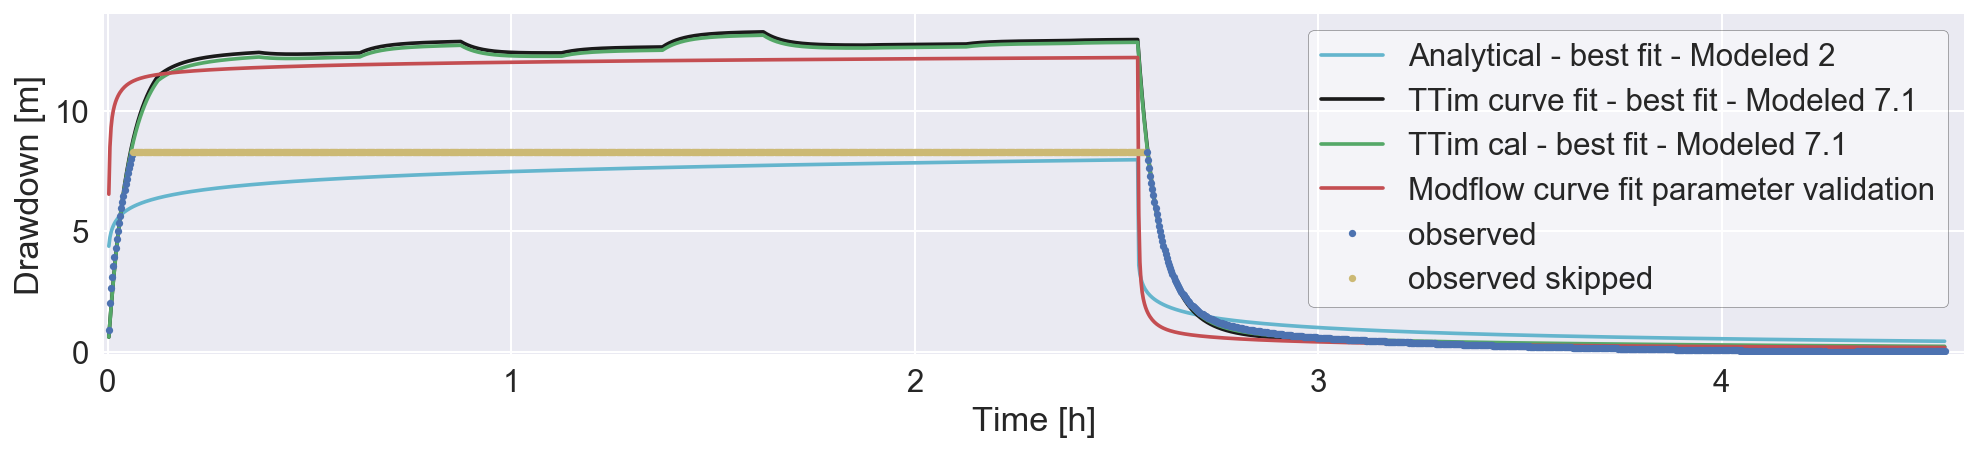
\includegraphics[width=1\linewidth]{bingo_1lay_analysis}
%		\captionsetup{justification=centering}		
%		\caption{\label{fig:bingo_1lay_analysis}}
%		\end{subfigure} \\ %\hfill
%	\begin{subfigure}[b]{1\linewidth}
%        \centering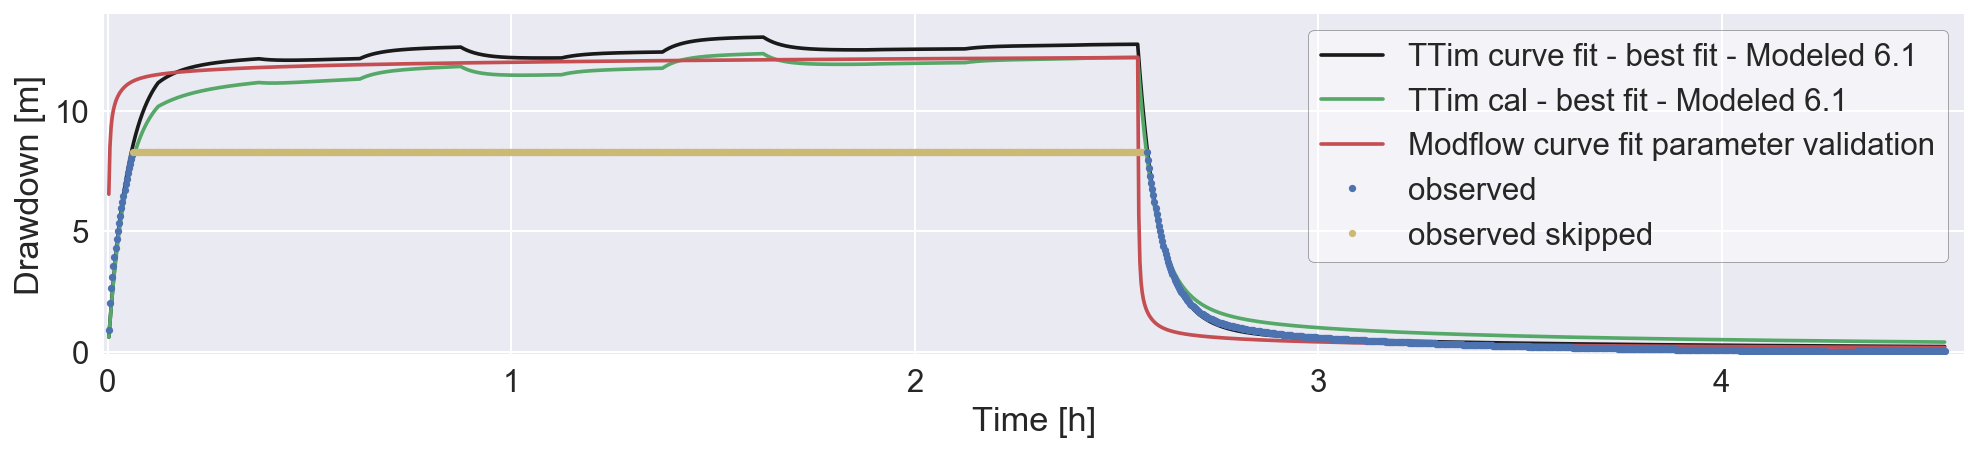
\includegraphics[width=1\linewidth]{bingo_2lay_analysis}
%		\captionsetup{justification=centering}		
%		\caption{\label{fig:bingo_2lay_analysis}}
%		\end{subfigure} \\
%	\begin{subfigure}[b]{1\linewidth}
%        \centering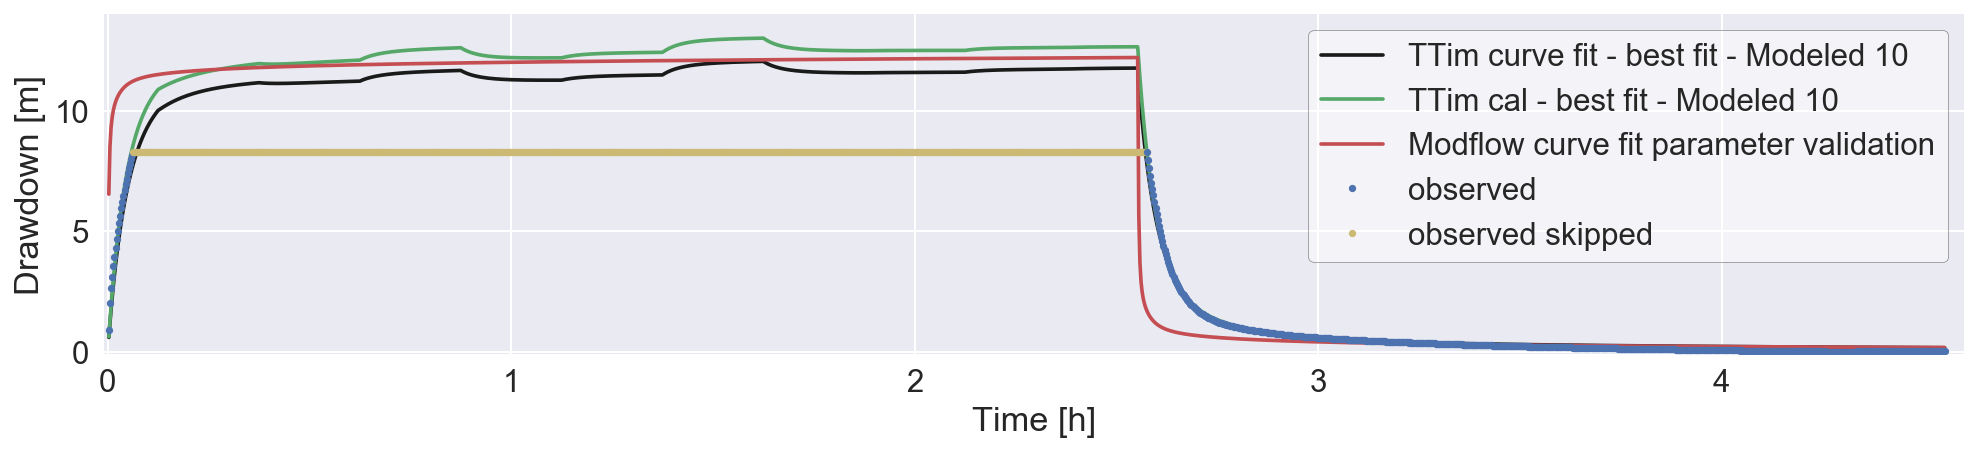
\includegraphics[width=1\linewidth]{bingo_3lay_analysis}
%		\captionsetup{justification=centering}		
%		\caption{\label{fig:bingo_3lay_analysis}}
%		\end{subfigure}
%	\captionsetup{justification=centering}	
%	\caption{Pumping test fit TS results: (\subref{fig:bingo_1lay_analysis}) single layered, ~(\subref{fig:bingo_2lay_analysis}) double layered and ~(\subref{fig:bingo_3lay_analysis}) triple layered (partially penetrating)} 
%	\label{fig:bingo_fieldwork_analysis}
%\end{figure} 

%
%\begin{table}[h!]
%\small
%\centering
%\caption{Bingo - overview best fit parameters}
%\label{tab:bingo_table}
%\begin{tabular}{l|l|l|lll|lll|l}
%\hline 
%\textbf{}       & \textbf{Stor [m]} & \textbf{Res [d]} & \textbf{T1}& \textbf{T2}  & \textbf{T3   [m$^2$/d]}  & \textbf{S1}& \textbf{S2}  & \textbf{S3 [-]}  & \textbf{RMSE [m]} \\ \hline
%\textbf{Single Lay}       & \textbf{} & \textbf{} & \textbf{}& \textbf{}& \textbf{}  & \textbf{}& \textbf{}& \textbf{}  & \textbf{}                    \\ \hline
%Analytical                & -             & -            & 10.83      & -          & -          & 2.0E-04    & -          & -          & 0.798         \\
%Curve fit                 & -             & 0.05         & 25.52      & -          & -          & 7.3E-05    & -          & -          & 0.166         \\
%Cal                       & -             & 2.5E-04      & 21.94      & -          & -          & 5.9E-19    & -          & -          & 0.175         \\
%{\textbf{}}               &               &              &            &            &            &            &            &            &               \\ 
%\textbf{Double Lay}       & \textbf{} & \textbf{} & \textbf{}& \textbf{}& \textbf{}  & \textbf{}& \textbf{}& \textbf{}  & \textbf{}                    \\ \hline
%Curve fit                 & -             & 0.06         & 22.88      & 0.40       & -          & 4.2E-04    & 8.0E-04    & -          & 0.167         \\
%Cal                       & -             & 0.02         & 11.63      & 0.57       & -          & 3.3E-07    & 4.7E-06    & -          & 0.413         \\ {\textbf{}}               &               &              &            &            &            &            &            &            &               \\ 
%\textbf{Triple Lay}       & \textbf{} & \textbf{} & \textbf{}& \textbf{}& \textbf{}& \textbf{}& \textbf{}& \textbf{}& \textbf{}                        \\ \hline
%Curve fit                 & -             & -            & 6.28       & 1.6E-03    & 0.86       & 1.8E-06    & 1.7E-02    & 2.0E-03    & 0.163         \\
%Cal                       & -             & -            & 17.95      & 3.76       & 3.35       & 0.18167    & 0.29988    & 0.11243    & 0.076         \\ \hline    
%\end{tabular}
%\end{table}

\subsection{Location: Nungo}

\textbf{Site inspection} \\
The remote community of Nungo is located in the Upper East Region (UER) of Ghana. Access is only possible by an unpaved road. The landscape is mildly sloping to flat. Low vegetation is interspersed by plains. Adjacent to the village an out of use agricultural field is present. The Volta river is located at approximately 400 m. Wet season flooding occurs due to riverbank over-topping. Inhabitants label inundation levels as extreme. Water levels of 3 m and higher persist for the entire rainy season. The infiltration well has perforations above surface level. At the moment of inspection the top of the well was deformed by heat, which meant it was not possible to close it of by a lid. \\
   
\textbf{Measurement quality} \\
Installation of the test set-up was affected by difficulties with pump immersion. From the first moment of pumping, discharge rates were effectively zero. An inspection revealed the well was filled with a liquid consisting of water, sandy clay and debris. The pumping test was restarted twice with an increased pump elevation. This did not result in an improvement. It was not possible to perform a pumping test at this location. \\
  
\textbf{Remark} \\
The well is clogged and should be cleaned before measurements can be done. No pumping test was performed and no data was acquired. 

\subsection{Location: Nyong Nayili}

\textbf{Site inspection} \\
The landscape of Nyong Nayili and its surroundings is mostly flat. A mix of bushes, low vegetation and crop fields is present. During site inspection, no agricultural fields had been delineated. The local community estimated that wet season inundation levels reach up to 1 m. Throughout the season inundation fluctuations occur, caused by rainfall. No river or water flow was observed in the area. A muddy, stagnant pond is present at close well range (approximately 40m). The infiltration bed was still inundated (approximately 0.2 m) during the pumping test. Well perforations were observed above the infiltration bed. The presence of water on the infiltration bed definitely had an impact on the measurements of the pumping test. \\

\textbf{Measurement quality} \\
The start of the pumping test was delayed because the well could not immediately be located, and because of a clogged discharge hose. Since nightfall was a time limiting factor, the delay resulted in a shortened total test duration. In addition, the inundated infiltration bed affected the pumping test. The first 20 minutes of drawdown measurements are affected by an (unknown) additional inflow (see Appendix \ref{chapter:fieldworkresults}). This period is not taken into account in further analysis. The noise of dripping water during pumping test application suggests the interference of additional inflow even beyond the first 20 minutes.  \\
 
\textbf{Fit analysis} \\
Theis's method encounters difficulties in finding  parameter values leading to a reasonable good fit. The optimal solution does not result in a reasonable curve fit. The resulting storativity is equal to the predefined upper bound. The solution is unreliable and can be neglected. The use of TTim has a positive impact on the outcome in data analysis. Found transmissivity values are not analogous, but potentially represent nature. The resulting storativity values can be interpreted as low. The obtained optimal borehole storage values are considerably high compared to the initial conditions. Values upto five times the actual borehole storage are encountered. These values potentially reflect the presence of additional inflow. Overall curve fitting performances are moderately good. The absence of a decent fit can potentially be attributed to the data that was left out and/or the unknown additional inflow of water over time. \\

\begin{table}[h!]
\small
\centering
\caption{Nyong Nayili - overview best fit parameters}
\label{tab:Nyong_Nayili_table}
\begin{tabular}{l|c|r|r|rr|rr|c}
\hline 
\textbf{}       & \textbf{Method} & \textbf{Stor [m]} & \textbf{Res [d]} & \textbf{T1}  & \textbf{T2   [m$^2$/d]}  & \textbf{S1}  & \textbf{S2 [-]}  & \textbf{RMSE [m]} \\ \hline \hline
Analytical                & fmin             & -             & -            & 6.00       & -          & 3.0e-01    & -          & 0.752 \\
1 lay                     & cal              & 0.2419        & -            & 13.35      & -          & 7.8e-05    & -          & 0.457 \\
2 lay                     & cal              & 0.2436        & -            & 6.95       & 6.98       & 4.6e-06    & 3.6e-05    & 0.457 \\
2 lay (pp)                & fmin             & 0.2659        & 1.7e-02      & 1.7e-04    & 28.61      & 1.1e-02    & 4.4e-06    & 0.450 \\ \hline    
\end{tabular}
\end{table}

\begin{figure}[h!]
 \centering
 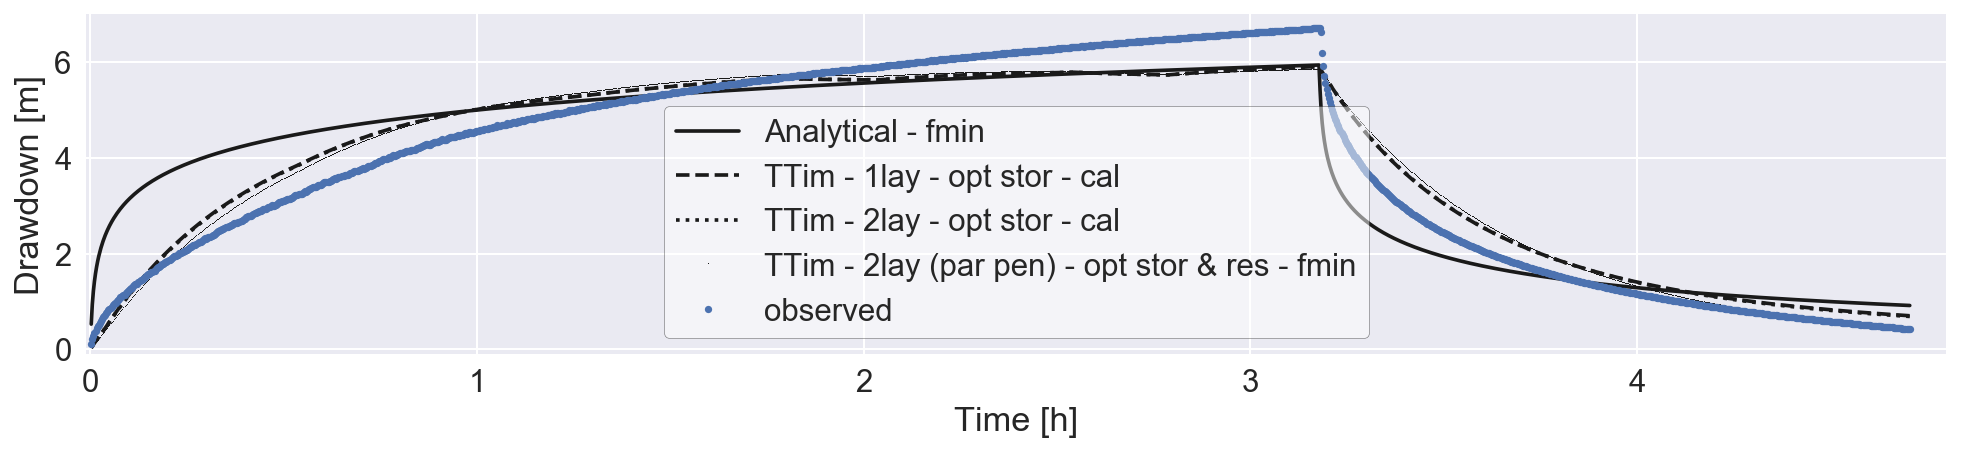
\includegraphics[width=\linewidth]{Nyong_Nayili_multi_lay_best}
 \captionsetup{justification=centering} 
 \caption{Nyong Nayili - Simplified models best fit}
 \label{fig:Nyong_Nayili_best}
\end{figure}

\textbf{Effect of model complexity} \\
The choice of optimization function did not significantly impact the values of the optimized parameters. An increase in the number of parameters did not improve model performance, it even worsens model performance in some cases. In all the model simulations the Root-Mean-Square-Error is substantial. The accuracy of the optimal parameter values is questionable. Further research on the impact of missing starting data and/or the impact of water inflow during a pumping test is recommended.  

\subsection{Location: Janga (1/2)}

\textbf{Site inspection} \\
The infiltration system near Janga is located at the bank of a dry river bed. The Volta river is located at approximately 1000 m (see fact-sheet visualisation, Appendix \ref{chapter:fieldworkresults}). A stagnant pond is present at a distance of approximately 70 m from the well. Wet season flooding is caused by the river. The flooding was described as a constant inundation of over 4 m and lasts for the the four months of wet season. During field visit no agricultural farm was seen. The infiltration well above surface level has perforations and is equipped with a plastic/concrete cover. \\ 

\textbf{Measurement quality} \\
Bush fires are frequent occurrences in the region. Due to close range appearance of fire at the time of measurement, the test is aborted early. The duration of the recovery process monitoring is affected. The color change in water discharged during the pumping test was noteworthy. The water switched color from brownish to grey to white to clear several times. \\

\textbf{Fit analysis} \\
The magnitude of the parameter is in line with the values found at the other research locations. The RMSE values are significantly larger, indicating the drawdown curve was not correctly modelled. The large RMSE-values can be attributed to the pumping test drawdown part. The shape of the drawdown curve shows an initial lowering of the groundwater level, which becomes more steady as time progresses. But then after approximately 90 minutes, the groundwater level starts dropping more quickly again before levelling off slightly.  None of the methods used in the analysis of the pumping test data is able to mimic the behaviour observed during this pumping test. \\

\begin{table}[h!]
\small
\centering
\caption{Janga first attempt - overview best fit parameters}
\label{tab:Janga1_table}
\begin{tabular}{l|c|r|r|rr|rr|c}
\hline 
\textbf{}       & \textbf{Method} & \textbf{Stor [m]} & \textbf{Res [d]} & \textbf{T1}  & \textbf{T2   [m$^2$/d]}  & \textbf{S1}  & \textbf{S2 [-]}  & \textbf{RMSE [m]} \\ \hline \hline
Analytical                & fmin             & -             & -            & 8.84       & -          & 3.0e-01    & -          & 1.339 \\
1 lay                     & fmin             & 0.0635        & -9.7e-03     & 9.09       & -          & 1.6e-02    & -          & 1.382 \\
2 lay                     & fmin             & 0.1287        & -            & 12.48      & 1.3e-04    & 1.9e-02    & 1.1e-08    & 1.445 \\
2 lay (pp)                & fmin             & 0.0635        & -            & 9.1e-05    & 15.19      & 4.3e-08    & 3.1e-03    & 1.530 \\ \hline    
\end{tabular}
\end{table}

\begin{figure}[h!]
 \centering
 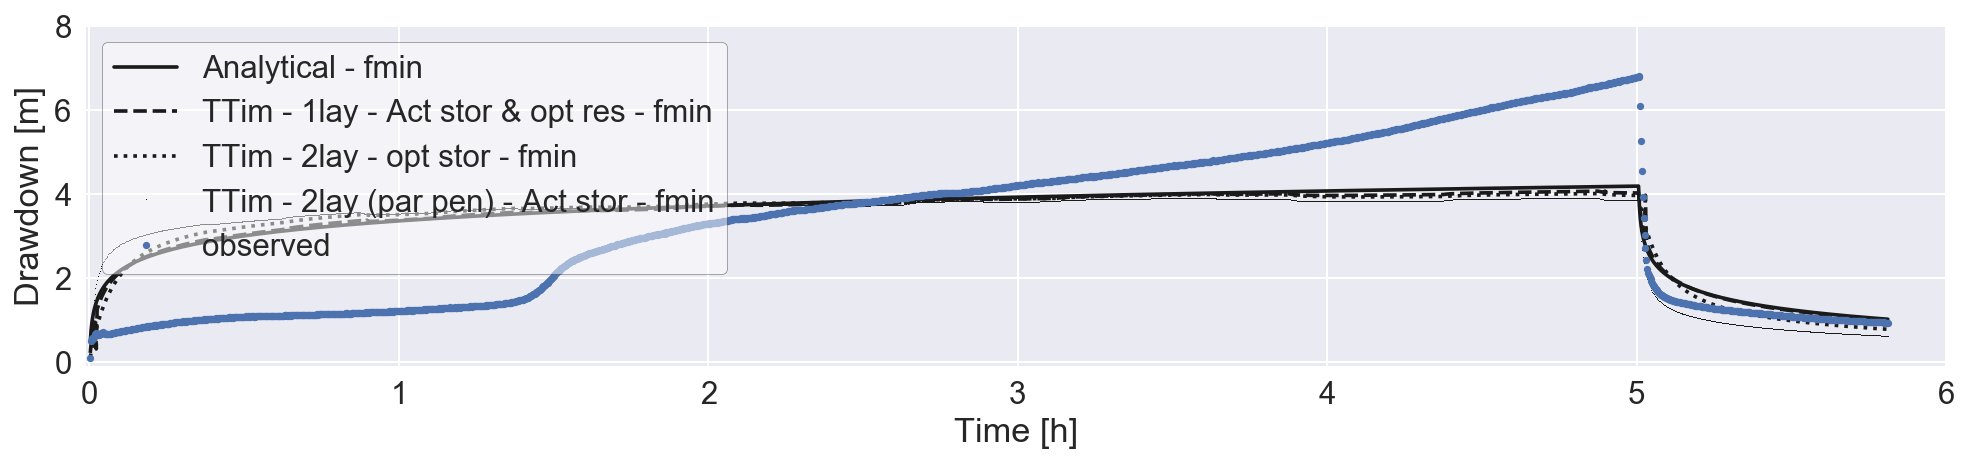
\includegraphics[width=\linewidth]{Janga1_multi_lay_best}
 \captionsetup{justification=centering} 
 \caption{Janga first attempt - Simplified models best fit}
 \label{fig:Janga1_best}
\end{figure}

\textbf{Effect of model complexity} \\
The shape of the drawdown curve is striking. There is a sudden increase in drawdown after 90 minutes of pumping. Towards the end of pumping period (four to five hours) the curve does not show the characteristic behaviour of reaching a new equilibrium. The variable rates of drawdown observed during the pumping test are not observed during the recovery test. As stated by \citet{Kruseman2000}, most of the time there is not a unique theoretical solution for these well-flow problems. This makes the identification of the right (theoretical) system even more difficult. Additional fieldwork could provide more information as to which local characteristics are causing this behaviour. A second pumping test was performed to verify whether the first test was done correctly.

\subsection{Location: Janga (2/2)}

\textbf{Measurement quality} \\
The initial (first two hours) pumping test discharge rates vary slightly (Appendix \ref{chapter:fieldworkresults}). The drawdown curve is potentially affected by these variations. Similar to the first test, the extracted water changed color several times. Compared to the previous research, the recovery period was monitored for longer. \\

\textbf{Fit analysis} \\
Despite the application of a pumping test with a lower discharge (compared to first attempt) the drawdown data shows similar behaviour. The lower values in Root-Mean-Square-Error can be attributed to the lower absolute drawdown (test with lower discharge rate) and the increased duration of recovery monitoring. The RMSE values still indicate the models are not able to describe the observed behaviour. The resulting parameters are shown in Table \ref{tab:Janga2_table}.

\begin{table}[h!]
\small
\centering
\caption{Janga second attempt - overview best fit parameters}
\label{tab:Janga2_table}
\begin{tabular}{l|c|r|r|rr|rr|c}
\hline 
\textbf{}       & \textbf{Method} & \textbf{Stor [m]} & \textbf{Res [d]} & \textbf{T1}  & \textbf{T2   [m$^2$/d]}  & \textbf{S1}  & \textbf{S2 [-]}  & \textbf{RMSE [m]} \\ \hline \hline
Analytical                & fmin             & -             & -            & 15.97      & -          & 3.0e-01    & -          & 0.571 \\
1 lay                     & fmin             & 5.4e-07       & -9.7e-03     & 13.54      & -          & 1.9e-02    & -          & 0.551 \\
2 lay                     & fmin             & 0.2228        & -2.2e-02     & 2.05       & 8.13       & 2.1e-02    & 4.1e-04    & 0.545 \\
2 lay (pp)                & fmin             & 0.2005        & -3.1e-02     & 6.59       & 0.86       & 9.4e-05    & 2.1e-03    & 0.545 \\ \hline    
\end{tabular}
\end{table}

\begin{figure}[h!]
 \centering
 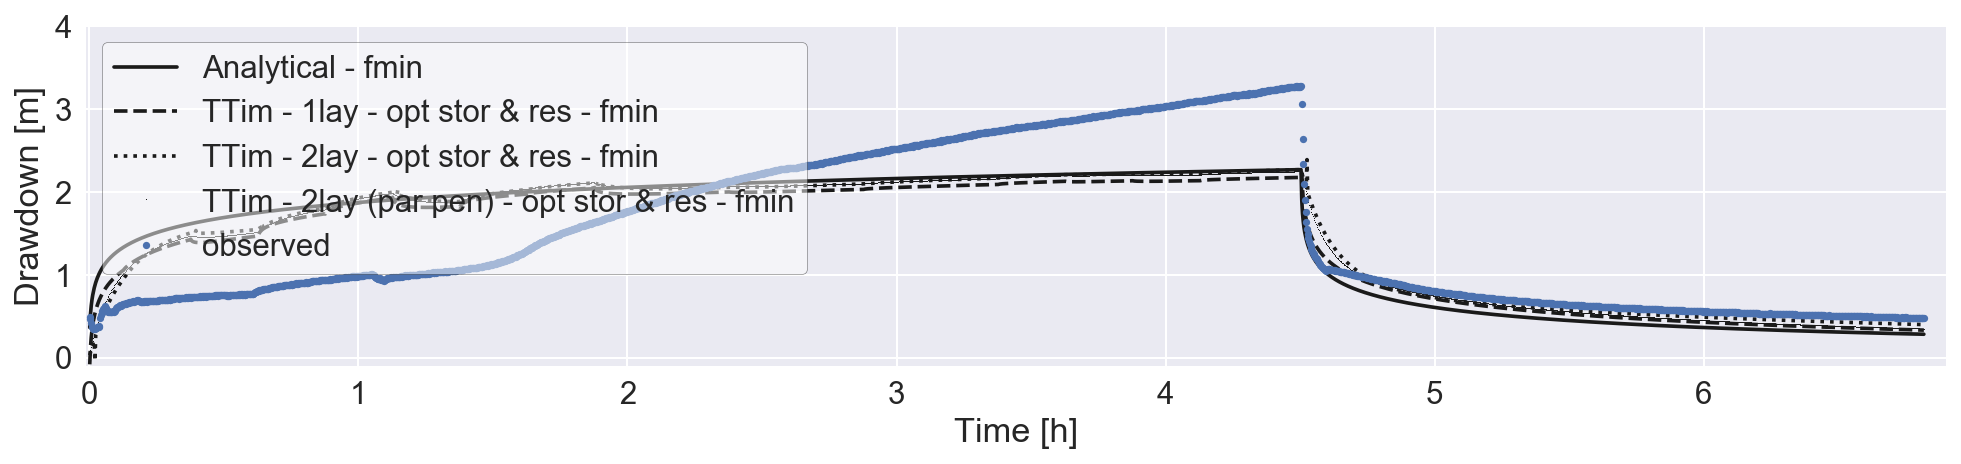
\includegraphics[width=\linewidth]{Janga2_multi_lay_best}
 \captionsetup{justification=centering} 
 \caption{Janga second attempt - Simplified models best fit}
 \label{fig:Janga2_best}
\end{figure}

\textbf{Effect of model complexity} \\
The second test confirms the behaviour observed in the first test. There are multiple explanations for this behaviour, i.e. one can think of the subsurface layers that are emptied as pumping continues, hydraulic interaction with the river bed or fracture zones drawdown and more. 
%Instead of further fieldwork investigation, it is advisable to gain knowledge in complex drawdwon data interpretation. 

\subsection{Location: Ziong (monitoring)}

\textbf{Site inspection} \\
In the study site surroundings of Ziong, no rivers, water flows or ponds were observed. Wet season inundation depths were said to be less than 2 m. Daily level variations occur as flooding is caused by rainfall. The landscape is flat. Occasionally, (bed)rock is observed at the surface. High grasses and bushes are present. There are several crop fields nearby. The infiltration system does not have perforations above surface level. A steel lid is present to cover the top of the well. The agricultural field and the ASR-system were fully operational. \\

\textbf{Measurement quality} \\
During the observed period the system was in daily operation. The system was monitored over multiple days. The divers had to be installed above the lowest groundwater levels because of the presence of the pump and the fact that the system was already in operation. This meant that the largest drawdowns could not be measured. The estimated discharge rate of 20 m$^3$/d is based on multiple measurements of the volume meter. In analysis it is assumed to be constant. The exact time at which the recovery starts is unknown because the lowest groundwater levels could not be measured. Based on the comparable test situation at the location Bingo, it is assumed the recovery starts 4 minuted before the first measurement indicating the recovery has started. \\
%Despite these defects the collected data can be used for further analysis.

\textbf{Fit analysis} \\
The analytical Theis method was not applied in this monitoring test situation. Analysis with TTim show reasonable results. The modelled drawdown corresponds closely with the observations. This example shows the advantages of TTim. The obtained transmissivity values of approximately 1 m$^2$/d are low. \\

\begin{table}[h!]
\small
\centering
\caption{Ziong - overview best fit parameters}
\label{tab:Ziong_table}
\begin{tabular}{l|c|r|r|rr|rr|c}
\hline 
\textbf{}       & \textbf{Method} & \textbf{Stor [m]} & \textbf{Res [d]} & \textbf{T1}  & \textbf{T2   [m$^2$/d]}  & \textbf{S1}  & \textbf{S2 [-]}  & \textbf{RMSE [m]} \\ \hline \hline
1 lay                     & fmin             & 0.0382        & -            & 1.76      & -         & 1.1e-03    & -          & 0.255 \\
2 lay                     & fmin             & 0.0635        & -0.05        & 0.38      & 1.05      & 2.9e-02    & 1.2e-03    & 0.240 \\
2 lay (pp)                & fmin             & 0.0147        & -0.08        & 0.23      & 0.78      & 2.6e-02    & 1.3e-03    & 0.243 \\ \hline    
\end{tabular}
\end{table}

\begin{figure}[h!]
 \centering
 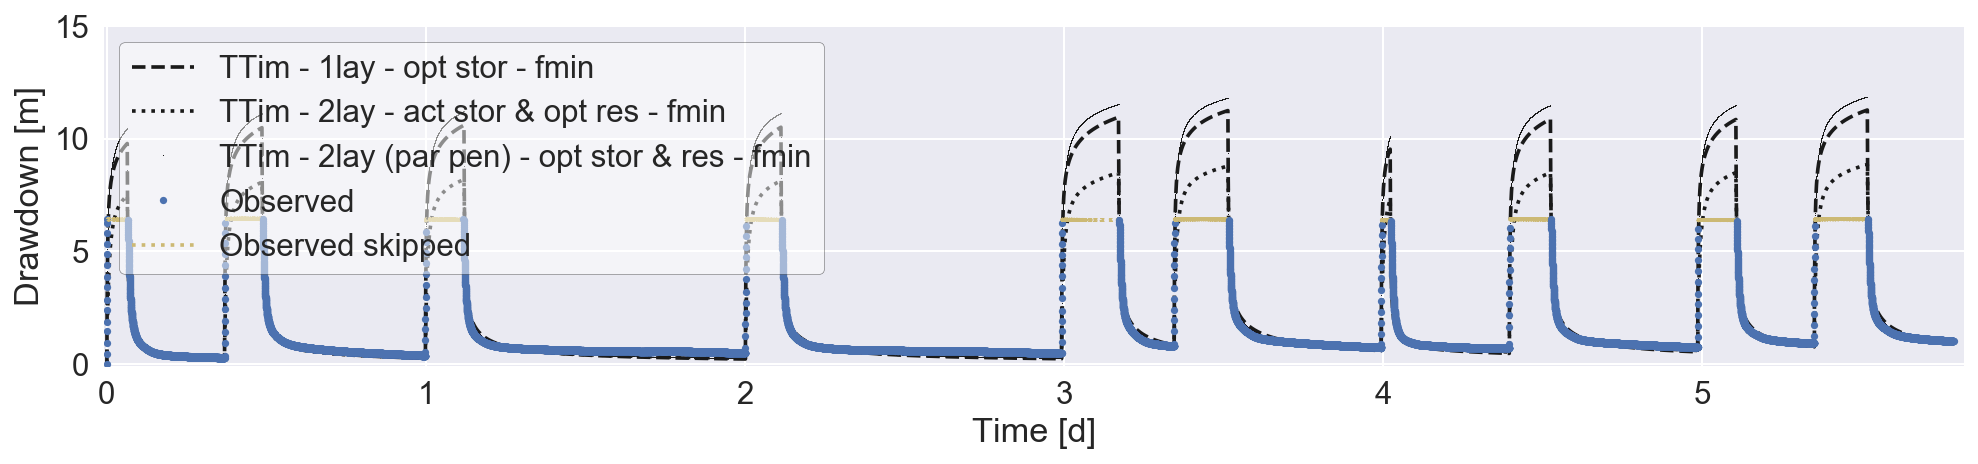
\includegraphics[width=\linewidth]{Ziong_multi_lay_best}
 \captionsetup{justification=centering} 
 \caption{Ziong - Simplified models best fit}
 \label{fig:Ziong_best}
\end{figure}

\textbf{Effect of model complexity} \\
Both optimization functions (\texttt{Fmin} and \texttt{Calibrate}) yield comparable parameters. When applying a simplified model with an increased number of degrees of freedom, the \texttt{Fmin} optimization function tends to score slightly better on values for the Root-Mean-Square-Error (Appendix \ref{chapter:Extense_fieldwork_analysis}). This however concerns a single measurement analysis, with a single set of predefined initial parameters. No other objective functions are taken into account. The performance of the different models does not show any trend. Models with an  increased number of degrees of freedom do not necessarily describe the observed data better. All three theoretical models are able to describe the observed data at Ziong to a certain extent. \\


%\section{Theoretical validation}
%
%\textbf{Soil analysis}
%
%\textbf{VES analysis}

\section{Results \& conclusions}
\label{section:fieldwork_conclusions}
This section contains the conclusions that can be drawn from the site visits and the analysis of pumping test data. The final part of this section describes how this data was used to derive parameters for soil scenarios to study potential methods for improvements of ASR systems in northern Ghana.  \\

\textbf{Maintenance of ASR systems}
\begin{itemize}
\item{ASR-system cleaning} \\
One year after construction (2016) the penetration depth of all five boreholes has decreased (significantly) due to the deposition of sand at the bottom of the well. The impact differs per location, but at each location a minimal depth decrease of 6 m is observed. The most striking example is the borehole at location Nungo, where a complete clogging has occurred (over 40 m decrease in depth). Measures should be taken to prevent the occurrence of clogging. It is recommended to seal of each borehole with a plastic/concrete lid. The tube penetrations above the infiltration bed should be sealed off permanently to avoid inflow of undesired sand and clay. In addition, annual maintenance of the borehole and infiltration bed is desirable.
         
\item{Additional research} \\
The results obtained through the analysis of the pumping tests seem to yield plausible estimates of subsurface characteristics. However, the models are not able to closely match the observations in all cases. Additional research could be done to expand the models to include processes that were left out in this analysis, e.g. inflow from the infiltration bed and irregularities (sudden additional decrease) in the drawdown time-series. Methods to deal with missing data (gaps in time series) could also be improved upon.
%
%Obtained pumping test drawdown data is potentially plausible. Nevertheless, uncertainty in the derivation of parameters and the selection of a (simplified) model consists. As stated by \citet{Kruseman2000}, additional fieldwork does not necessarily solve these uncertainties. No new comparable pumping tests at the same borehole locations are needed at short term. Gaining knowledge on the interpretation of data can possibly offer solutions. Complementary research on how to deal with gabs in pumping test data and/or irregularities in drawdown time-series is advisable. Moreover, future research can be pointed at the impact of (time-dependent) inflow of water during pumping test application. 

\item{Recommendations for future pumping tests} \\
Pumping tests should be performed with at least one (preferably more) observation well at a certain distance from the well \citep{Kruseman2000}. These tests potentially give insight in well skin behaviour (degree of resistance) and increase the amount of data from which subsurface parameters can be derived. The installation of one or more divers is recommended if complete ASR system understanding is required. This can provide more insight into how these system function throughout the year.

\end{itemize}

\textbf{Applicability of methods \& models}
\begin{itemize}
\item{Performance (analytical) methods; Theis \& TTim} \\
Compared to the simplest pumping test interpretation (Theis's method), TTim offers more model options (borehole storage, well skin resistance, multiple layers) in drawdown data analysis \citep{Mishra2013,Bakker2013}. In this research TTim outperforms Theis's method. However, TTim also encounters limitations, e.g. when there is a variable inflow at the start of a pumping test or when an additional sudden drop in drawdown occurs. 

\item{Performance of optimization functions; \texttt{Fmin} \& \texttt{Calibrate}} \\
Obtained geohyrological parameters represent local nature to a certain extend. This is confirmed by the Root-Mean-Square-Error values (objective function). Application of the two optimization functions generates outcomes. The results of different optimization functions can lead to ences in parameter size, while goodness of the fit statistics (RMSE) are comparable. However, the resulting parameters are generally similar. Therefore, it can be concluded that both optimization functions (\texttt{Fmin} and \texttt{Calibrate}) are applicable for the determination of suitable $T$ and $S$ values. 

\item{Performance of proposed subsurface models}  \\
Three simplified system models were used: a single layer model, a double layer model and a model with two layers and partial penetration of the well (Figure \ref{fig:Schematic_1lay_analysis} - \ref{fig:Schematic_3lay_analysis}). Based on the Root-Mean-Square-Error objective function, none of these systems performs consistently better or worse than any of the others. Therefore, the most simple (the single layer) model is applied in the rest of this research.
\end{itemize}

\textbf{$T$ \& $S$ values} \\
Drawdown measurements are taken in the extraction well. This set-up deviates from the desired common standard \citep{Kruseman2000}. It should be kept in mind that the quality of the data can be questioned. At each location different combinations of parameters yielded similar drawdown curves. This is likely a consequence of only having measurements inside the extraction well. The different models that were applied in the analysis of the data did not yield significantly different results. It is clear that due to the lack of groundwater measurements in the vicinity of the pumping wells, there is some uncertainty in the derived subsurface parameters. \\

The results from Bingo are used in further analysis. A bandwidth is defined to deal with the uncertainties mentioned in Section \ref{section:TS}. Upper and lower limits for $T$ and $S$ values are derived. The bandwidth is presented in Figure \ref{fig:Parameter_bandwidth}. Transmissivity limits are based on the obtained values in Section \ref{section:TS} and some factor of safety. For the definition of the storativity values a different approach was used. The  parameters limits are based on more commonly found  values. The chosen lower limit storativity ($S_{lower}$) corresponds with the situation of a confined aquifer, while the upper limit ($S_{upper}$) related more to the specific yield of a phreatic storage \citep{Strack1989,Fitts2012}. \\

\begin{figure}[h!]
 \centering
 
\includegraphics[width=0.6\linewidth]{Parameter_bandwidth_large}
 \captionsetup{justification=centering} 
 \caption{$T$ \& $S$ bandwidth selection}
 \label{fig:Parameter_bandwidth}
\end{figure}

%The defined scope can not be interpreted as a generalization of the different locations. Not a single combination of the upper and lower parameter boundaries is the one-on-one representation of a specific location. The bandwidth predominantly acts as an input for scenario modelling in the subsequent parts of this research. Outcome of these scenarios are perhaps quantitatively incorrect, but can qualitatively be interpreted as indication for the impact of ASR-system improvements within northern Ghana. 

